\section{MPS}
\label{s:mps}

\subsection{Abstract Syntax}

Structures represent abstract syntax tree nodes in MPS \cite{pech2013jetbrains}.
In \autoref{fig:mps/structure/fsm} the fsm structure is pictured.
It extends the abstract context expression from the base language.
This enables the fsm node to be used later as an Java expression.
The other nodes are defined the same way.

\begin{figure}[H]
	\centering
	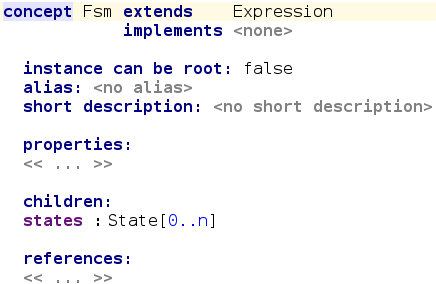
\includegraphics[width=0.7\textwidth]{structure_fsm.png}
	\caption{Structure for the Fsm Node in MPS} 
	\label{fig:mps/structure/fsm}
\end{figure}

\subsection{Concrete Syntax}

The concrete syntax for the FSML is defined by editors for the abstract syntax.
This reflects the projectional nature of MPS \cite{pech2013jetbrains}.
In \autoref{fig:mps/editor/fsm} the cell layout contains the fsm keyword and a vertical collection of cells representing the states of the fsm.

\begin{figure}[H]
	\centering
	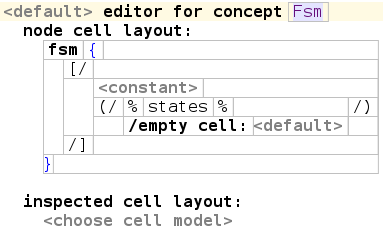
\includegraphics[width=0.7\textwidth]{editor_fsm.png}
	\caption{Editor for the Fsm Structure in MPS} 
	\label{fig:mps/editor/fsm}
\end{figure}

\subsection{Constraints}

Constraints with custom error or warning messages are built by defining non-typesystem rules \cite{mpspatterns}.
The non-typesystem rule in \autoref{fig:mps/constraint/fsm} applies to the fsm abstract syntax tree node.
Each unreachable state node in the fsm a warning is generated.

\begin{figure}[H]
	\centering
	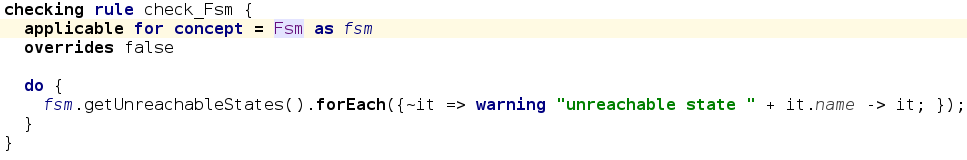
\includegraphics[width=\textwidth]{constraint_fsm.png}
	\caption{Non-typesystem Rule for the Fsm Structure in MPS} 
	\label{fig:mps/constraint/fsm}
\end{figure}

\subsection{Code Generation}

The code generator uses reduction rules to transform the FSML structures to the MPS Base Language.
Optionally reduction rules can be applied based on conditions.
Ultimately the code generator uses the MPS Base Language to generate Java source code.

\autoref{fig:mps/reduction/fsm} shows the reduction rule for the fsm node. 
The template on the right side represents the creation of a new \lstinline{Fsm} object.

\begin{figure}[H]
	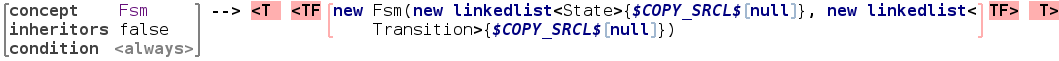
\includegraphics[width=\textwidth]{reduction_rule_fsm.png}
	\caption{Reduction Rule for the Fsm Structure in MPS}
	\label{fig:mps/reduction/fsm}
\end{figure}

\subsection{Tests}

MPS provides a DSL for testing language implementations.
\autoref{fig:mps/tests/fsm} illustrates the negative test case for the reachable state condition. 
This is done by indicating that a cell in the editor should contain an error or warning.
In this case the \lstinline{stateC} cell is expected to contain the \lstinline{UnreachableState} warning.


\begin{figure}[H]
	\centering
	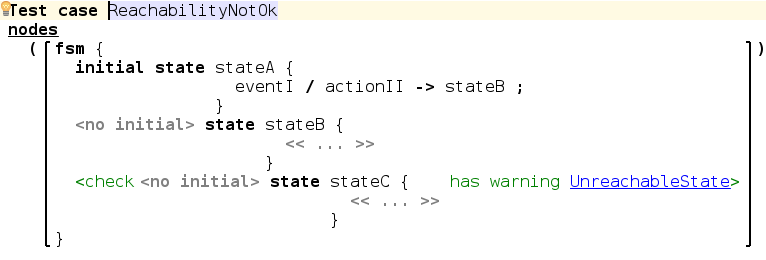
\includegraphics[width=\textwidth]{test_fsm.png}
	\caption{Tests in MPS} 
	\label{fig:mps/tests/fsm}
\end{figure}
